\documentclass{article}%
\usepackage{amsfonts}
\usepackage{longtable}
\usepackage{amsmath}
\usepackage{amssymb}
\usepackage{graphicx}%
\setcounter{MaxMatrixCols}{30}
\providecommand{\U}[1]{\protect\rule{.1in}{.1in}}
%EndMSIPreambleData
\newtheorem{theorem}{Theorem}
\newtheorem{acknowledgement}[theorem]{Acknowledgement}
\newtheorem{algorithm}[theorem]{Algorithm}
\newtheorem{axiom}[theorem]{Axiom}
\newtheorem{case}[theorem]{Case}
\newtheorem{claim}[theorem]{Claim}
\newtheorem{conclusion}[theorem]{Conclusion}
\newtheorem{condition}[theorem]{Condition}
\newtheorem{conjecture}[theorem]{Conjecture}
\newtheorem{corollary}[theorem]{Corollary}
\newtheorem{criterion}[theorem]{Criterion}
\newtheorem{definition}[theorem]{Definition}
\newtheorem{example}[theorem]{Example}
\newtheorem{exercise}[theorem]{Exercise}
\newtheorem{lemma}[theorem]{Lemma}
\newtheorem{notation}[theorem]{Notation}
\newtheorem{problem}[theorem]{Problem}
\newtheorem{proposition}[theorem]{Proposition}
\newtheorem{remark}[theorem]{Remark}
\newtheorem{solution}[theorem]{Solution}
\newtheorem{summary}[theorem]{Summary}
\newenvironment{proof}[1][Proof]{\noindent\textbf{#1.} }


\begin{document}
\title{Shakespeare and Satoshi : using embeddings and LSTM to metricize
authorship}
\author{Micah Warren\\University of Oregon}
\maketitle


\begin{abstract}
We train an LSTM for next word prediction, using embeddings for authors of the work as well as word-embedding.   After training, we analyze the Euclidean metric on the embedding space for the authors.  We use data provided by Ramesh and Watson \cite{RWgithub} in which a classifier was trained.  Several experiments are repeated, and the metrics appear, upon inspection, to be somewhat consistent between experiments.  In comparing Shakespeare works to disputed Shakespeare works, our method recovers the correct result in several cases.  Our metrics suggest that, among the potential Satoshi candidates given in \cite{RW} Gavin Andreson's writing is the closest to that of Satoshi Nakamoto.
\end{abstract}

\section{Introduction}


In this note, we report on experiments which follow the experiments
in \cite{RW}. \ In \cite{RW} a neural network is trained on known data
attributed to known authors, and then this is used to predict authorship of works written by 
unknown or disputed authors. \ The methods are applied to disputed or apochryphal
Shakespeare works.   The methods are also applied to emails from the real Satoshi Nakamoto as well as a number
of prominent Satoshi suspects.  For more background on these authorship problems and stylometry, see \cite{RW}. For a book on stylometry applied to Shakespeare, see \cite{M}.  For an interesting stylometric attempt to identify Satoshi, see \cite{SG}.

\ \ In this note, using the same data set, we
take a different approach. For Shakespeare, we train an LSTM to predict the next word in a sequence,
while feeding in both a word embedding and a embedding of each work, disputed
or not. After the embeddings have been trained for some time, we extract the
Euclidean distance on the embeddings of the works. \ The works of the different
authors Shakespeare, Marlowe, etc, appear to cluster. \ The disputed works
attributed to Shakespeare do appear to lie near the works nowadays attributed to
him. \ We feel this is promising. \ 


The method of data analysis we use is first multi-dimensional scaling to get a two-dimensional projection of the points, followed by old-fashioned eyeballing.  Color-coded pictures make eyeballing an easy task.  

For Satoshi, we perform similar experiments, reading emails or forum posts  from each of the
authors and trying to predict the next word, using an embedding vector of the
author as input. After training, we compare the embedding vector of Satoshi to
the other authors (using the eyeball method described above.) We perform a number of experiments as the training is somewhat random. A pattern does emerge.  The data
suggests that Andreson is most likely.  Some other authors appear unlikely, including ``faketoshi'' Craig
Wright as well as Nick Szabo, thus our results disagree with the more supervised approach in \cite{SG}. See Tables 1,2.  

\section{More details: Shakespeare}

The cleaned data, generously provided by the authors of \cite{RW} at
\cite{RWgithub} is where we start. \ \ There are 33 different works we consider:
24 works with undisputed authors include Shakespeare, Jonson, Marlowe, Dekker
and Middleton, and 9 works which are unlabeled. \ \ For this data set
\textit{Pericles} \ was split into multiple acts as the authorship is believed
to be mixed. \ In each experiment, the cleaned data was broken into chunks of
8 or more consecutive words in a sentence. Each training sample consisted of 8
consecutive words together with the work they were from, and the target variable is the
next word. \ Both the words and the work were put into separate embeddings,
the words into embeddings of varying dimensions, and the works
into space of varying (lower) dimensions. \ \ These were trained for several hours each in several experiments. 
The network architecture is as follows.  Both word embeddings and work embedding are fed into an LSTM layer with 64 dimensions of output.  A dropout of 0.1 is added, then a dense 64 ReLU layer before the softmax output layer.    
\ Using MDS we took the distance functions of the embedding vectors of each work
and viewed these in two dimensions, which are seen in the pictures in the following pages.  

\section{Shakespeare: Pictures}

Comments on the pictures are given in captions.  Overall we observe the experiments are fairly similar and consistent.   During the experiments we renormalized the weights so that they stayed on the unit sphere.  (Without doing this, occasionally unfortunate clusters appear at the origin - on the other hand there's plenty of room to move about the unit sphere. )  Thus the pictures of embeddings in lower dimensions can appear to lie near the unit circle.  (In particular, Experiment 3 exhibits this effect.)  

We ran the experiments for different amounts of time and varied some other hyperparameters, including embedding dimension of both the words and the work. The point of this note isn't to study the nuances of choosing hyperparameters for this approach, rather to demonstrate how embedding can place individual authors in a larger latent metric space of authors. 


\section{Comparison with Reality}

It is believed \cite{M} that Shakespeare wrote the final 3 acts of \emph{Pericles}.   According to our analysis, he would be quite likely responsible for \emph{iv} and possibly for the other acts.   The other suspected author, George Wilkins is not in this data set.  

\emph{Birth of Merlin} is attributed to William Rowley, also not in this author set.  

\emph{Thomas Lord Cromwell} is nowadays not attributed to Shakespeare. Several authors have been suggested although none are considered in this set. 

\emph{The Puritan} is attributed to Middleton \cite{H}.  Our metrics concur.  


 \emph{Vortigern and Rowena} is attributed well-known forger William Henry Ireland.    Looking at the above pictures, one may be tempted to conclude Marlowe was the author.  As we aren't using any test samples from Ireland, this shouldn't be considered a failure of the method.  

\section{Satoshi}

The process for identifying Satoshi was similar.  We took data in \cite{RWgithub} which is given in the form of scraped emails, blog and forums post from Satoshi as well as from 10 well-known early experts in cryptocurrency see \cite[section 3.1.2]{RW}.  

We trained with shorter sentences (only length 5) as well as longer sentences.  The pictures follow.  We point out the pictures are more misleading here then in the Shakespeare case:  Because MDS must try to optimize the distance between all sets of point, it is easy to poorly represent the distance from a certain point.  So while one can visually see from inspection that Gavin Andreson is often the closest, this is much more clear when you look at the distance squared matrix.   We sum up the distance squared matrix over the length 5 sentences and then the longer sentences, and present these first in tables 1 and 2.  MDS images follow.  

In \cite{RW} the classifier estimated that most of Satoshi's work would be attributed to Andreson, if given a choice among the suspects.   The authors suggest that the preponderance of training samples coming from Andreson may bias the classification toward Andreson.   In our case, we would only have to worry about this sort of bias if the winner lies in the ``center'' of the metric space, that is, is close to a lot of the others, not just Satoshi. However, we can observe, visually in the pictures as well as in the tables, that such an issue does not arise.  More importantly, it seems that both Satoshi and Andreson appear to frequently lie on the outer parts of the image.  In most of the cases, Satoshi and Andreson are linearly separable in the two dimensional picture (that is, we can separate them from the rest of the group by drawing a line.)  This happens rarely for Satoshi with other authors. 




\begin{thebibliography}{999}





\bibitem{SG}  Grey, Skye (1 December 2013). \emph{Satoshi Nakamoto is (probably) Nick Szabo } 
https://likeinamirror.wordpress.com/2013/12/01/satoshi-nakamoto-is-probably-nick-szabo/

\bibitem{H}Hamilton, Donna B.  intoduction in
 \emph{Thomas Middleton and Early Modern Textual Culture}, ed. Taylor and Lavagnino. Oxford University Press, 2007.  358–359.
  
\bibitem{M}
  MacDonald P. Jackson.
  \emph{Defining Shakespeare: Pericles as Test Case}.
   Oxford University Press, 2003

\bibitem{RW}
  Ramesh, Varun and Watson, Jean-Luc.
  \emph{Shakespeare and Satoshi - De-anonymizing Writing Using BiLSTMs with Attention}.
   2018.  
   https://web.stanford.edu/class/archive/cs/cs224n/cs224n.1184/reports/6858026.pdf
  

\bibitem{RWgithub}  Ramesh, Varun and Watson, Jean-Luc.   
https://github.com/jlwatson/cs224n-project


\end{thebibliography}


\begin{figure}
\noindent\makebox[\textwidth]{%
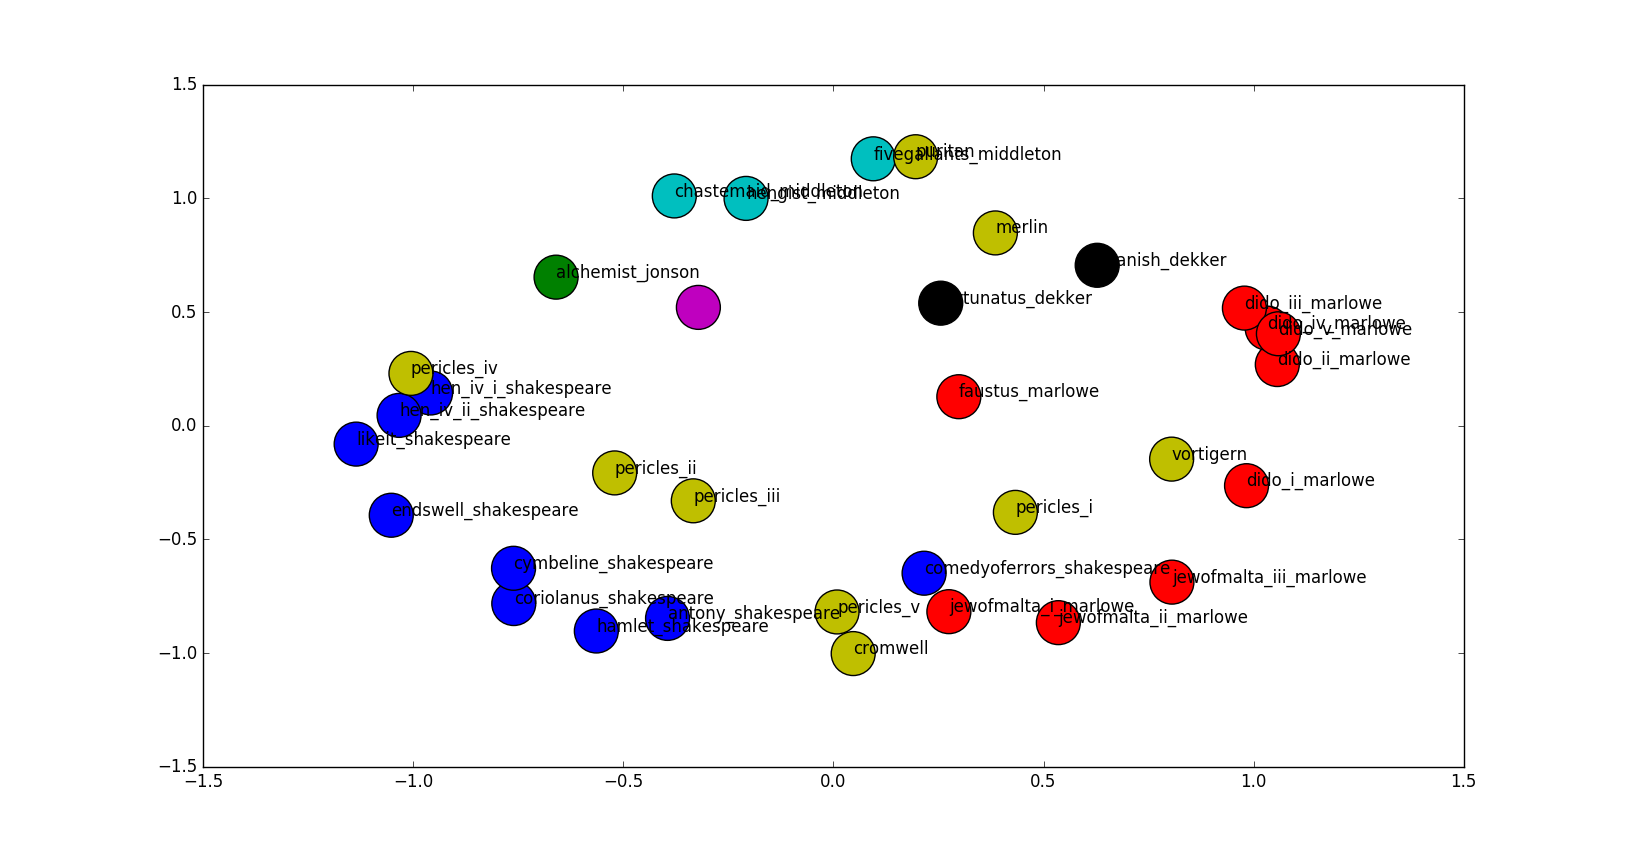
\includegraphics[width=1.4\textwidth]{experiment1}}
\caption{Experiment 1 : 8 dimensional work embedding, 80 dimensional word embedding,  8 hour training.  Minimum sentence length is 8.
As we see, a satisfying clustering occurs: Shakespeare appears to lie in the
lower left corner, Marlowe on the right side, Middleton near the top, and the
two Dekker works near each other and in between Middleton and Marlowe, Jonson
is also somewhat isolated. \ \ (The purple point was a null input accidently
left in the first experiment. ) We also note that \textit{puritan}, which is attributed to Middleton, would
clearly be attributed to Middleton upon inspection of the above picture (top center.) Vortigern, which is attributed to William Henry Ireland, appears to be
Marlowe, however William Henry Ireland was not an author in this data set.
 }
\end{figure}


\begin{figure}
\noindent\makebox[\textwidth]{%
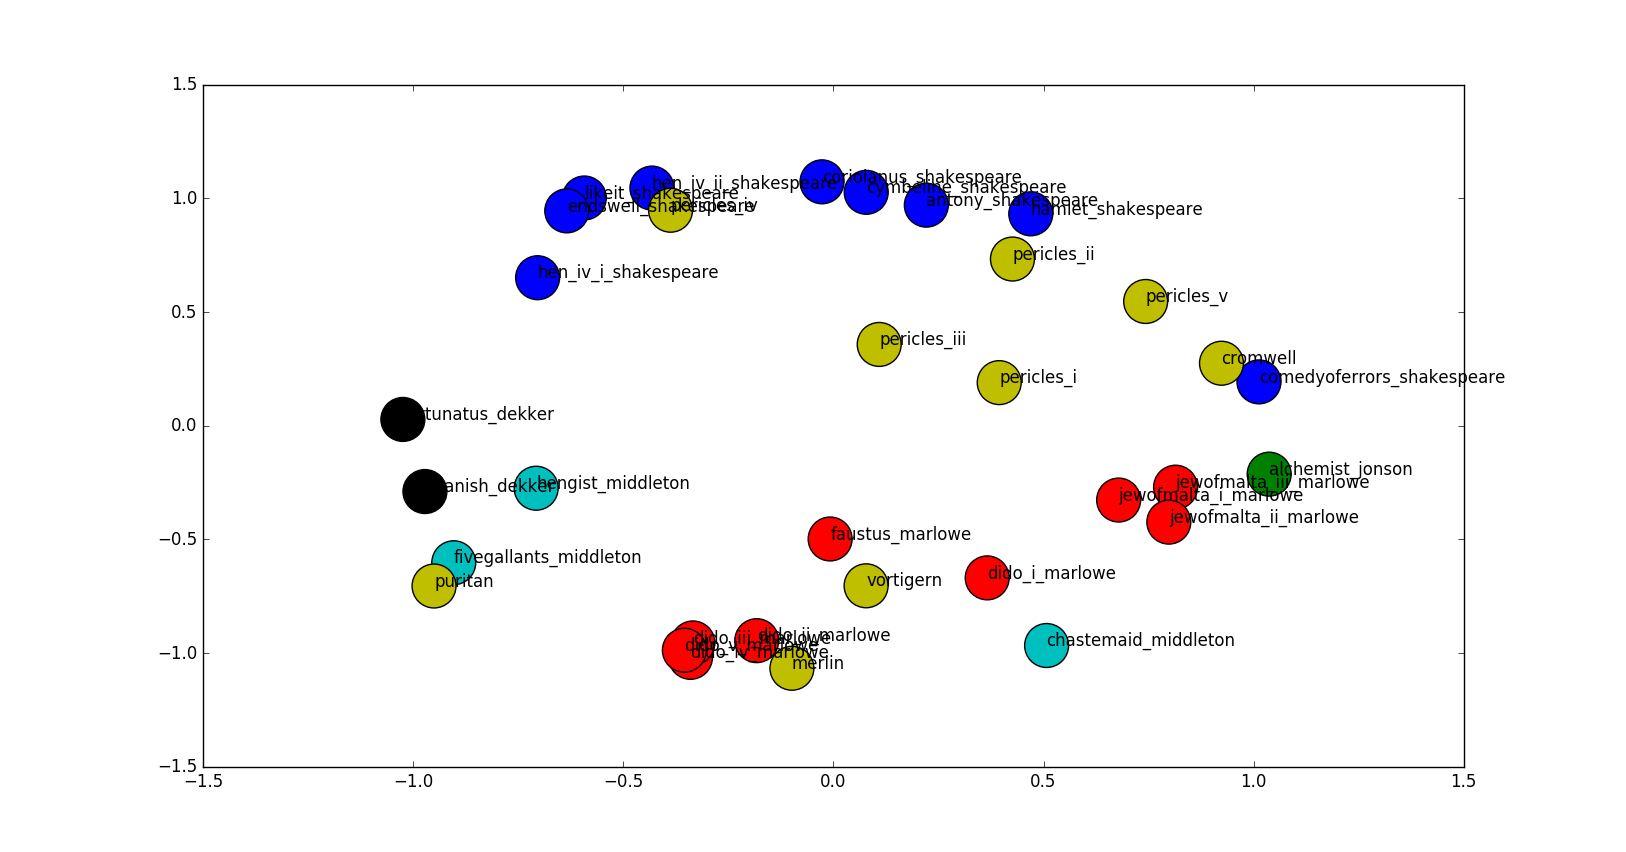
\includegraphics[width=1.4\textwidth]{experiment2}}
\caption{Experiment 2 : 5 dimensional work embedding, 50 dimensional word embedding, 7 hour training. Minimum sentence length is 8.}
\end{figure}


\bigskip


\begin{figure}
\noindent\makebox[\textwidth]{%
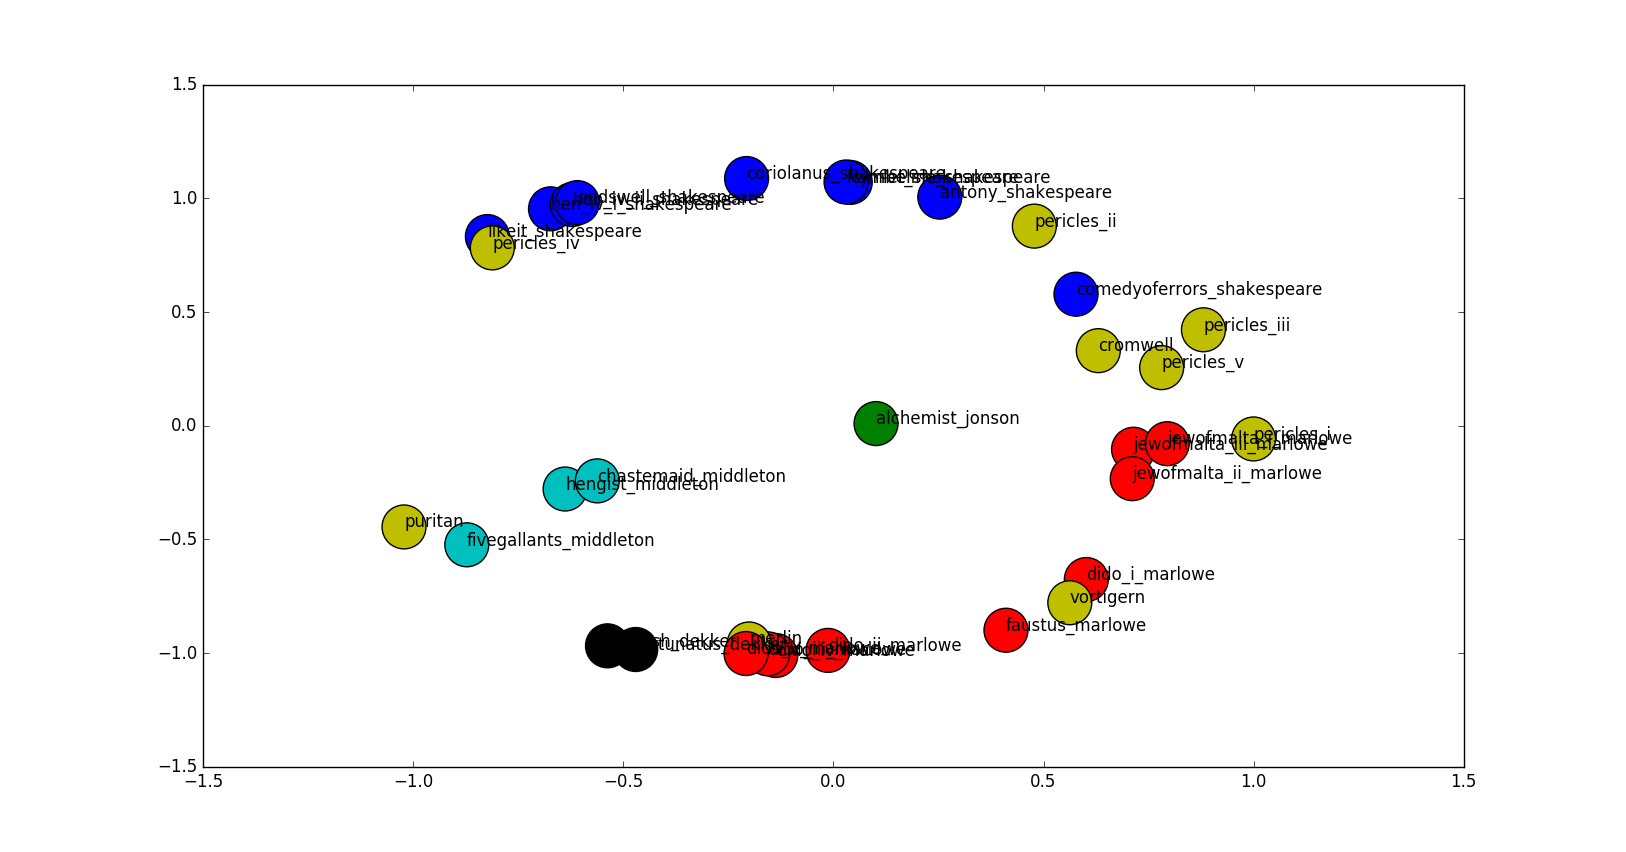
\includegraphics[width=1.4\textwidth]{experiment3}}
\caption{Experiment 3: 3 dimensional work embedding, 40 dimensional word embedding, 4 hour training.  Minimum sentence length is 8. The normalization effect before MDS is easy to see in dimension 3. }
\end{figure}



\bigskip


\begin{figure}
\noindent\makebox[\textwidth]{%
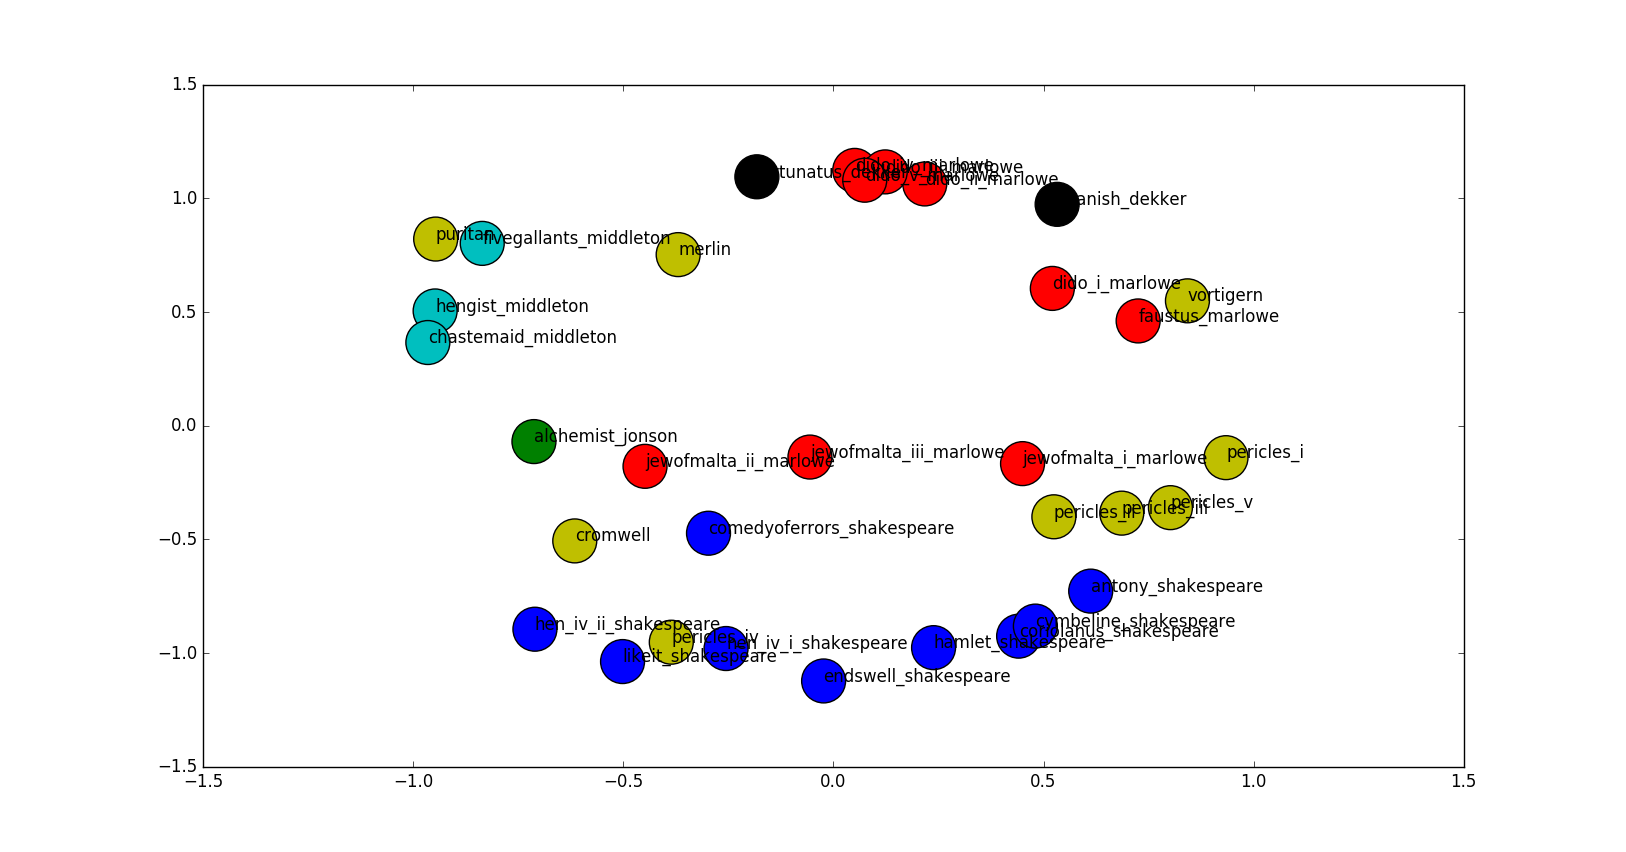
\includegraphics[width=1.4\textwidth]{experiment4}}
\caption{Experiment 4: 6 dimensional work embedding, 50 dimensional word embedding, trained for 90 minutes. Minimum sentence length is 8.}
\end{figure}


\bigskip

\begin{figure}
\noindent\makebox[\textwidth]{%
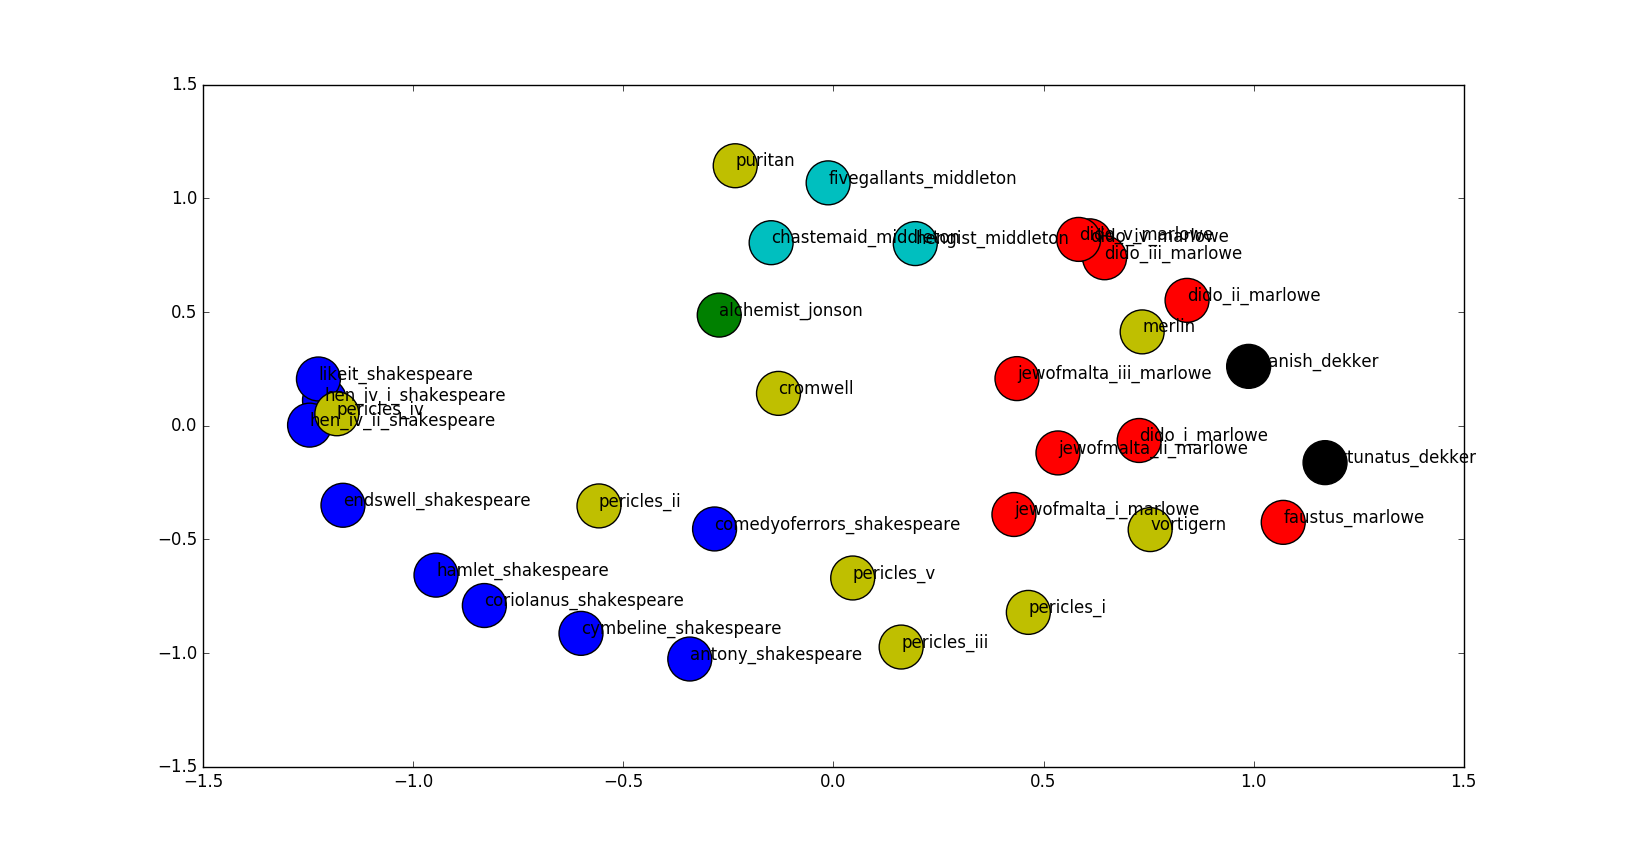
\includegraphics[width=1.4\textwidth]{experiment5_10_hours}}
\caption{Experiment 5: 4/70 dimensional work/word embeddings.  Minimum sentence length is 8. Trained for 10 hours. }
\end{figure}
\begin{figure}
\noindent\makebox[\textwidth]{%
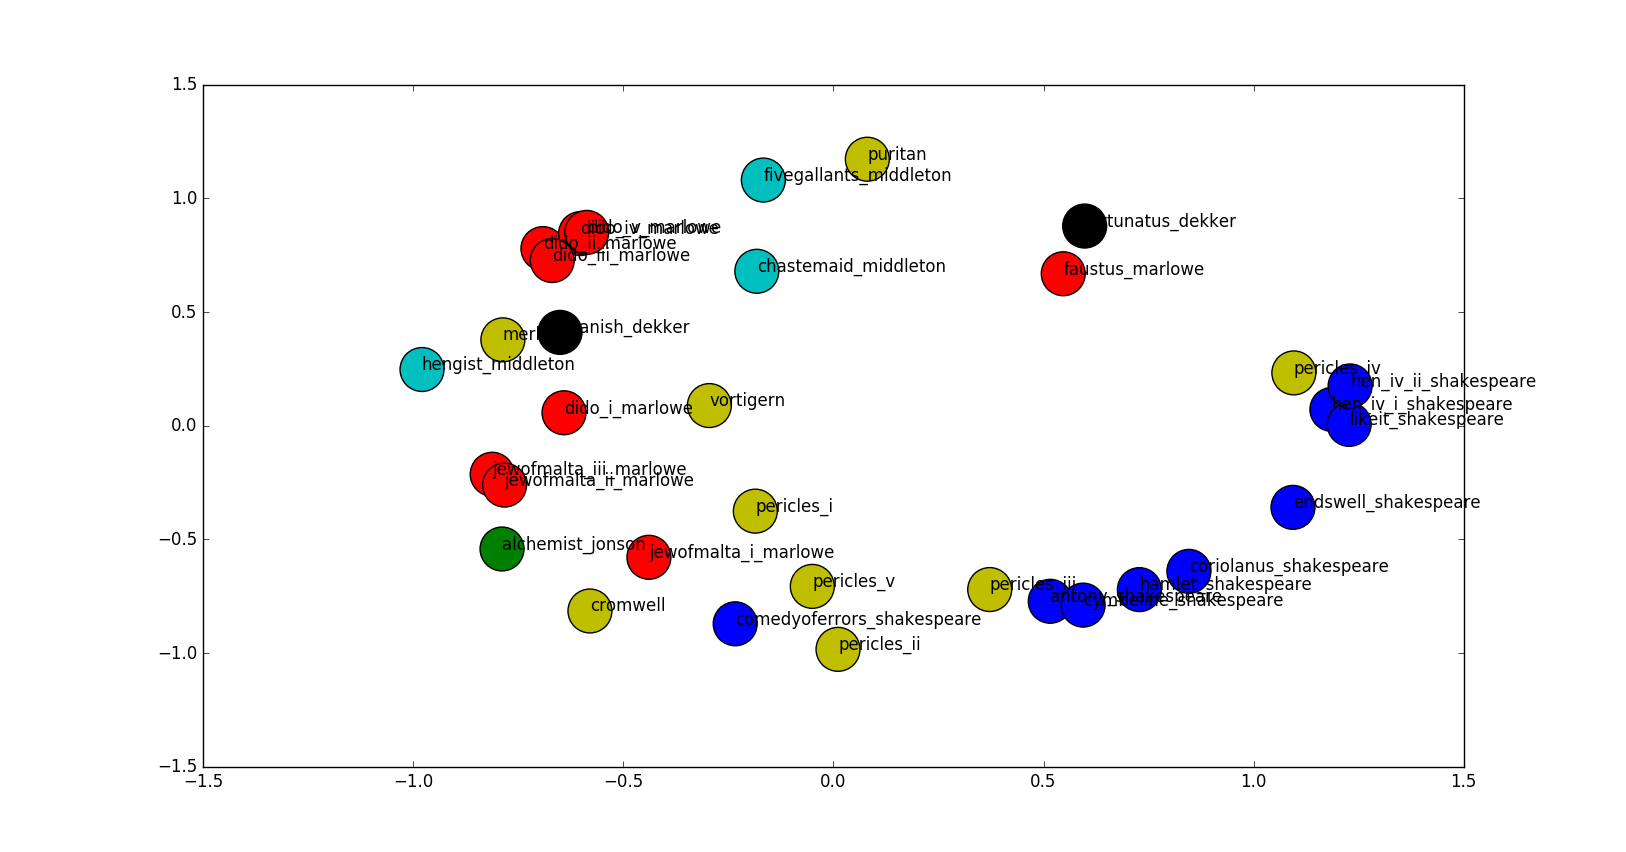
\includegraphics[width=1.4\textwidth]{experiment5_3hoursin}}
\caption{Experiment 5: 4/70 dimensional work/word embeddings.  Minimum sentence length is 8. This is the same experiment but picture was after 3 hours.   There are a few dissimilarities- these could be partially due to the loss of information in the MDS projections.  }
\end{figure}



\bigskip

\begin{figure}
\noindent\makebox[\textwidth]{%
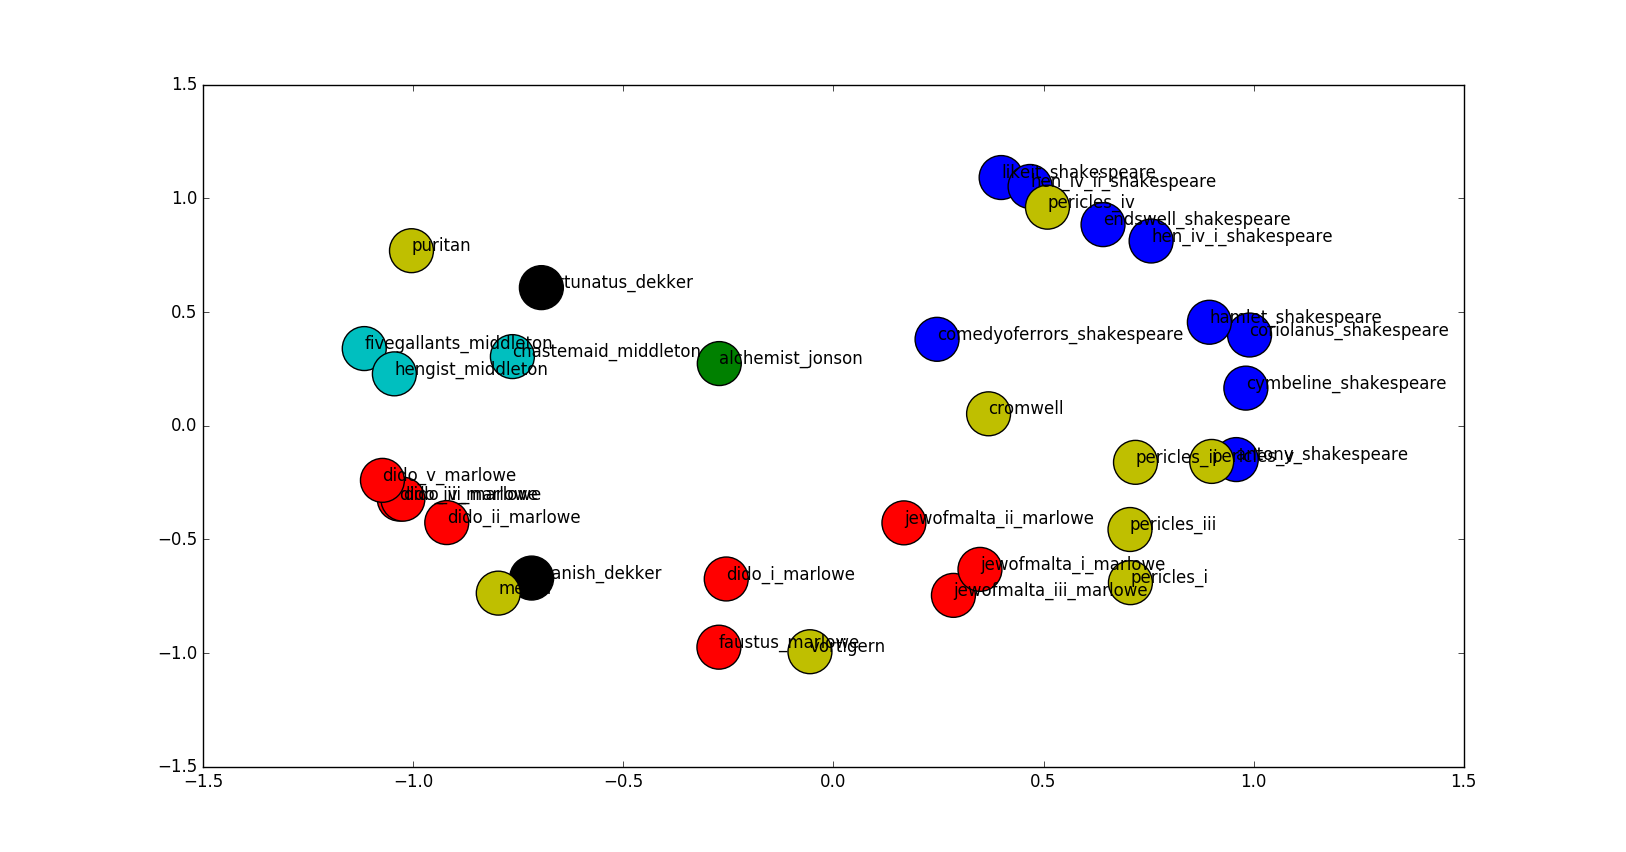
\includegraphics[width=1.4\textwidth]{experiment6}}
\caption{Experiment 6: 5/65 dimensional work/word embeddings.  Minimum sentence length is 8. Trained for 3 hours.}
\end{figure}

\begin{figure}
\noindent\makebox[\textwidth]{%
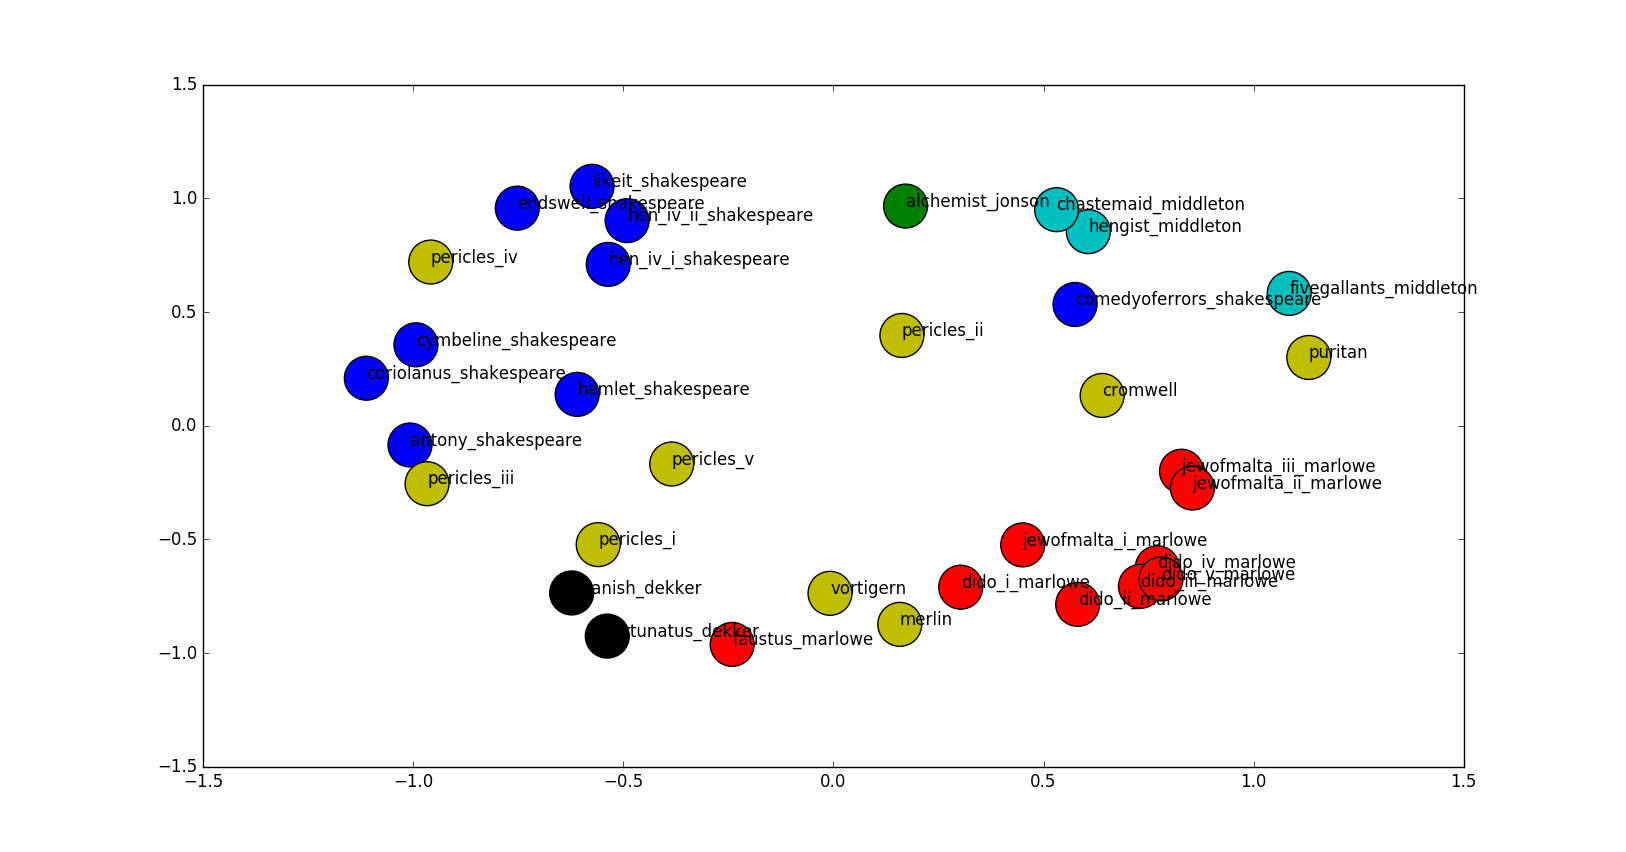
\includegraphics[width=1.4\textwidth]{experiment7}}
\caption{Experiment 7: 5/65 dimensional work/word embeddings.  Minimum sentence length is now 3. Trained for 12 hours.}
\end{figure}


\begin{figure}
\noindent\makebox[\textwidth]{%
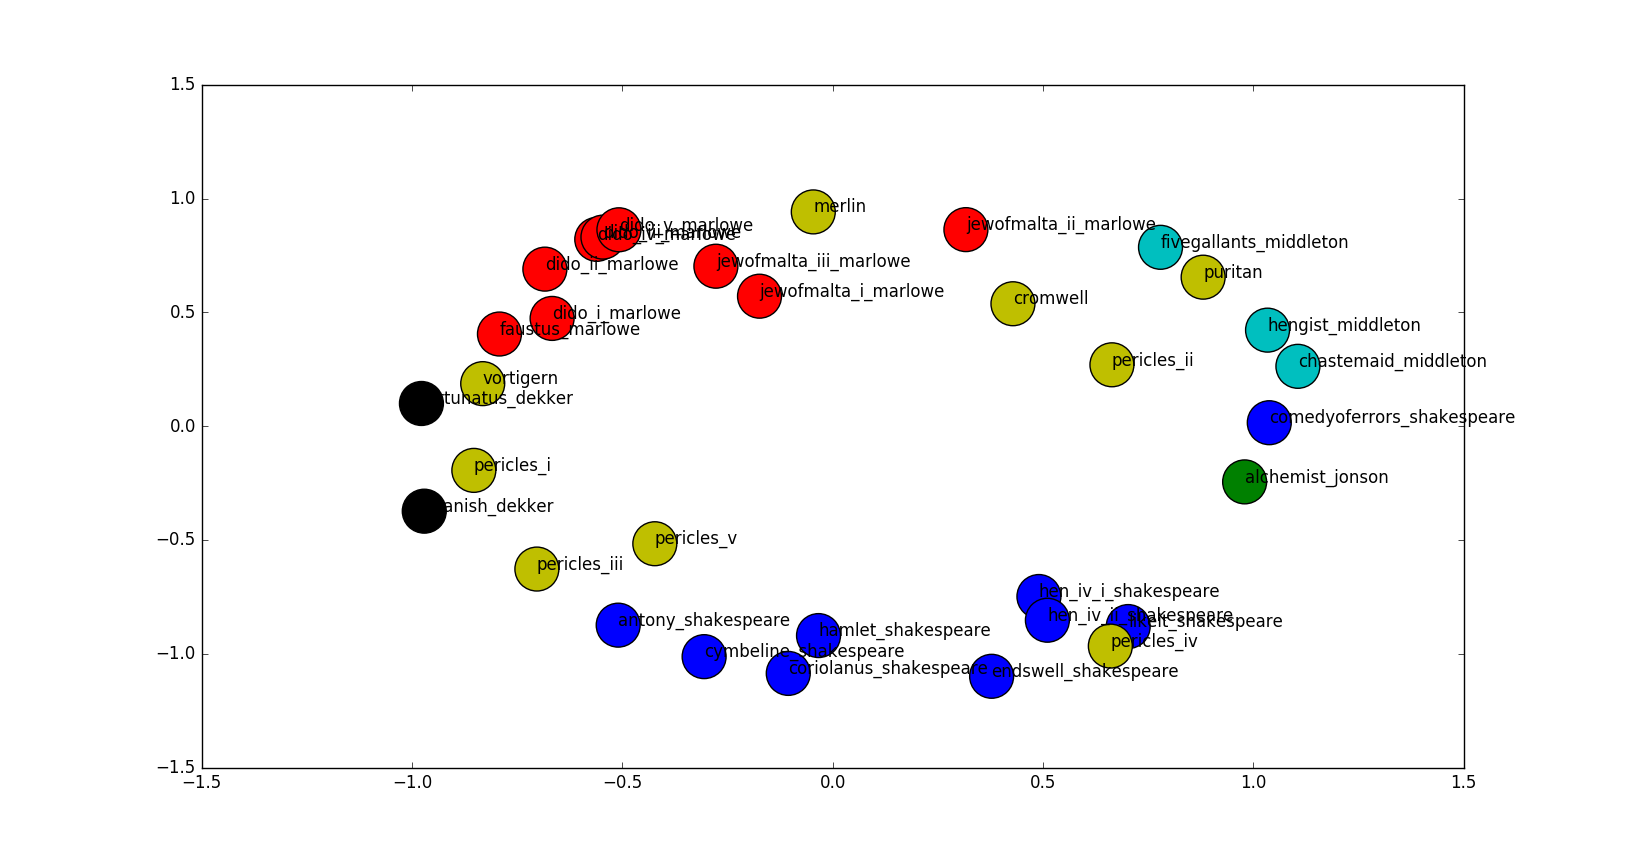
\includegraphics[width=1.4\textwidth]{experiment8}}
\caption{Experiment 8: Same as experiment 7.  5/65 dimensional work/word embeddings.  Minimum sentence length is now 3. Trained for 12 hours.}
\end{figure}


\begin{table}[]
\begin{tabular}{llll}
author              & dorian-nakamoto & gavin-andresen & craig-steven-wright \\
dorian-nakamoto     & 0               & 15.17    & 21.70         \\
gavin-andresen      & 15.17     & 0              & 18.63        \\
craig-steven-wright & 21.70    & 18.63    & 0                   \\
nick-szabo          & 24.66     & 33.90    & 29.38         \\
hal-finney          & 20.23     & 20.42   & 16.45        \\
satoshi-nakamoto    & 14.82     & 3.38    & 18.41         \\
david-mazieres      & 16.44     & 15.84     & 19.53         \\
micheal-clear       & 17.46     & 20.71     & 4.82          \\
wei-dai             & 21.95     & 22.22  & 11.45        \\
roger-ver           & 5.70    & 11.44    & 14.48        \\
jed-mccaleb         & 8.15     & 6.29    & 13.82        \\
                    & nick-szabo      & hal-finney     & satoshi-nakamoto    \\
dorian-nakamoto     & 24.67    & 20.23    & 14.82         \\
gavin-andresen      & 33.90     & 20.42351439    & 3.380080909         \\
craig-steven-wright & 29.38511904     & 16.45340055    & 18.40573374         \\
nick-szabo          & 0               & 25.64857474    & 34.56030691         \\
hal-finney          & 25.64857474     & 0              & 11.41229908         \\
satoshi-nakamoto    & 34.56030691     & 11.41229908    & 0                   \\
david-mazieres      & 28.54803643     & 2.178079683    & 7.259632932         \\
micheal-clear       & 29.5008966      & 18.06477784    & 19.8159157          \\
wei-dai             & 26.90783671     & 27.75107912    & 25.12389958         \\
roger-ver           & 30.95822402     & 18.71143656    & 13.19109422         \\
jed-mccaleb         & 34.32852304     & 14.3267214     & 6.565597684         \\
                    & david-mazieres  & micheal-clear  & wei-dai             \\
dorian-nakamoto     & 16.44428568     & 17.46368376    & 21.95114888         \\
gavin-andresen      & 15.8390849      & 20.7133555     & 22.21610074         \\
craig-steven-wright & 19.52788978     & 4.81742211     & 11.44949844         \\
nick-szabo          & 28.54803643     & 29.5008966     & 26.90783671         \\
hal-finney          & 2.178079683     & 18.06477784    & 27.75107912         \\
satoshi-nakamoto    & 7.259632932     & 19.8159157     & 25.12389958         \\
david-mazieres      & 0               & 19.11397549    & 27.0450094          \\
micheal-clear       & 19.11397549     & 0              & 7.844918806         \\
wei-dai             & 27.0450094      & 7.844918806    & 0                   \\
roger-ver           & 16.46900615     & 11.49533086    & 18.73847202         \\
jed-mccaleb         & 11.57167203     & 13.19747908    & 22.56449224         \\
                    & roger-ver       & jed-mccaleb    &                     \\
dorian-nakamoto     & 5.703376187     & 8.148551639    &                     \\
gavin-andresen      & 11.44136401     & 6.287780197    &                     \\
craig-steven-wright & 14.47920723     & 13.81882883    &                     \\
nick-szabo          & 30.95822402     & 34.32852304    &                     \\
hal-finney          & 18.71143656     & 14.3267214     &                     \\
satoshi-nakamoto    & 13.19109422     & 6.565597684    &                     \\
david-mazieres      & 16.46900615     & 11.57167203    &                     \\
micheal-clear       & 11.49533086     & 13.19747908    &                     \\
wei-dai             & 18.73847202     & 22.56449224    &                     \\
roger-ver           & 0               & 2.484674678    &                     \\
jed-mccaleb         & 2.484674678     & 0              &                    
\end{tabular}

\caption{Sum of distance-squared matrices, over all length 5 sentence experiments}
\end{table}



\begin{table}[]
\begin{tabular}{llll}
author              & dorian-nakamoto & gavin-andresen & craig-steven-wright \\
dorian-nakamoto     & 0               & 3.895719897    & 4.659285647         \\
gavin-andresen      & 3.895719897     & 0              & 4.316430826         \\
craig-steven-wright & 4.659285647     & 4.316430826    & 0                   \\
nick-szabo          & 4.96642144      & 5.822795697    & 5.42080428          \\
hal-finney          & 4.497851586     & 4.519238253    & 4.056279151         \\
satoshi-nakamoto    & 3.84967459      & 1.838499635    & 4.290190409         \\
david-mazieres      & 4.055155445     & 3.979834783    & 4.4190372           \\
micheal-clear       & 4.178957258     & 4.551192756    & 2.194862663         \\
wei-dai             & 4.685205319     & 4.713395882    & 3.38371075          \\
roger-ver           & 2.388174237     & 3.382508538    & 3.805155349         \\
jed-mccaleb         & 2.854566804     & 2.507544655    & 3.717368536         \\
                    & nick-szabo      & hal-finney     & satoshi-nakamoto    \\
dorian-nakamoto     & 4.96642144      & 4.497851586    & 3.84967459          \\
gavin-andresen      & 5.822795697     & 4.519238253    & 1.838499635         \\
craig-steven-wright & 5.42080428      & 4.056279151    & 4.290190409         \\
nick-szabo          & 0               & 5.064442194    & 5.878801486         \\
hal-finney          & 5.064442194     & 0              & 3.378209448         \\
satoshi-nakamoto    & 5.878801486     & 3.378209448    & 0                   \\
david-mazieres      & 5.343036256     & 1.475831861    & 2.6943706           \\
micheal-clear       & 5.431472783     & 4.250267973    & 4.451507127         \\
wei-dai             & 5.187276425     & 5.267929301    & 5.012374645         \\
roger-ver           & 5.564011504     & 4.325671805    & 3.6319546           \\
jed-mccaleb         & 5.859054791     & 3.785065574    & 2.562342226         \\
                    & david-mazieres  & micheal-clear  & wei-dai             \\
dorian-nakamoto     & 4.055155445     & 4.178957258    & 4.685205319         \\
gavin-andresen      & 3.979834783     & 4.551192756    & 4.713395882         \\
craig-steven-wright & 4.4190372       & 2.194862663    & 3.38371075          \\
nick-szabo          & 5.343036256     & 5.431472783    & 5.187276425         \\
hal-finney          & 1.475831861     & 4.250267973    & 5.267929301         \\
satoshi-nakamoto    & 2.6943706       & 4.451507127    & 5.012374645         \\
david-mazieres      & 0               & 4.371953281    & 5.200481651         \\
micheal-clear       & 4.371953281     & 0              & 2.800878221         \\
wei-dai             & 5.200481651     & 2.800878221    & 0                   \\
roger-ver           & 4.058202329     & 3.390476494    & 4.328795678         \\
jed-mccaleb         & 3.401716042     & 3.632833479    & 4.750209705         \\
                    & roger-ver       & jed-mccaleb    &                     \\
dorian-nakamoto     & 2.388174237     & 2.854566804    &                     \\
gavin-andresen      & 3.382508538     & 2.507544655    &                     \\
craig-steven-wright & 3.805155349     & 3.717368536    &                     \\
nick-szabo          & 5.564011504     & 5.859054791    &                     \\
hal-finney          & 4.325671805     & 3.785065574    &                     \\
satoshi-nakamoto    & 3.6319546       & 2.562342226    &                     \\
david-mazieres      & 4.058202329     & 3.401716042    &                     \\
micheal-clear       & 3.390476494     & 3.632833479    &                     \\
wei-dai             & 4.328795678     & 4.750209705    &                     \\
roger-ver           & 0               & 1.576285088    &                     \\
jed-mccaleb         & 1.576285088     & 0              &                    
\end{tabular}

\caption{Sum of distance-squared matrices, over all length 8 experiments}
\end{table}




\begin{figure}
\noindent\makebox[\textwidth]{%
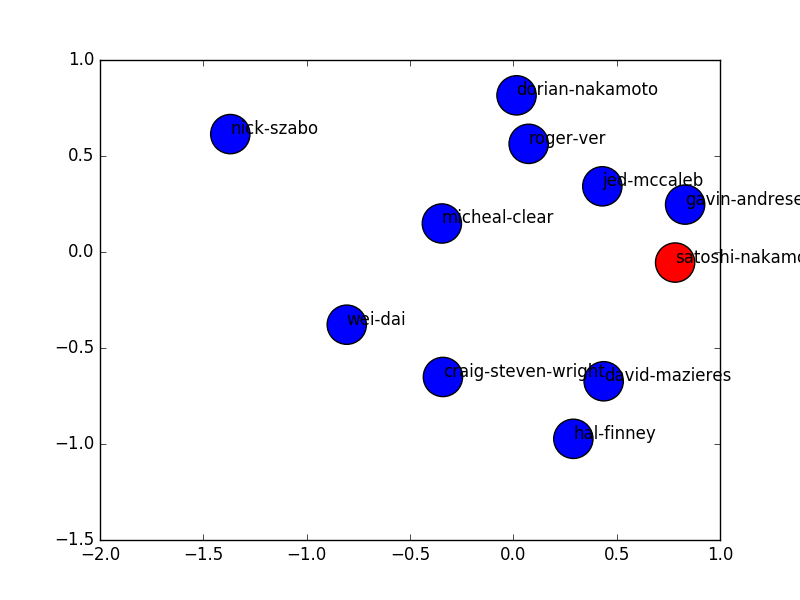
\includegraphics[width=1.4\textwidth]{figure_1}}
\caption{Experiment 1: 4 dimensional author embedding, 85 dimension word embedding, trained for 24 hours. Minimum sentence length is 5}
\end{figure}


\begin{figure}
\noindent\makebox[\textwidth]{%
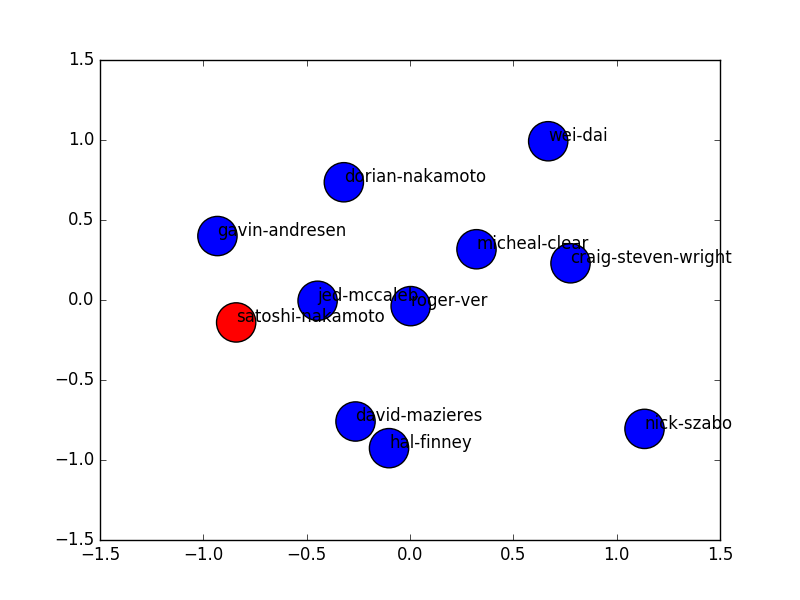
\includegraphics[width=1.4\textwidth]{figure_2}}
\caption{Experiment 2: 6 dimensional author embedding, 85 dimension word embedding, trained for 18 hours. Minimum sentence length is 5}
\end{figure}

\begin{figure}
\noindent\makebox[\textwidth]{%
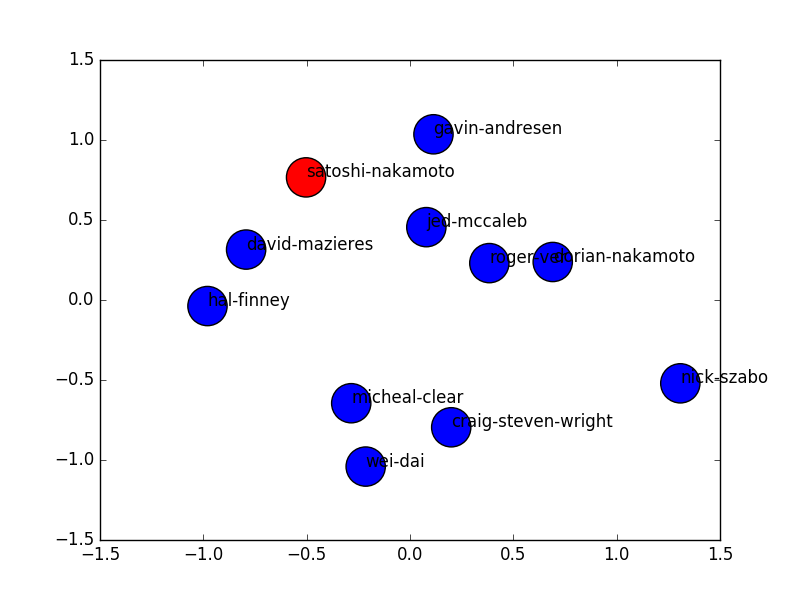
\includegraphics[width=1.4\textwidth]{figure_3}}
\caption{Experiment 3: 7 dimensional author embedding, 95 dimension word embedding, trained for 48 hours. Minimum sentence length is 5}
\end{figure}
\begin{figure}
\noindent\makebox[\textwidth]{%
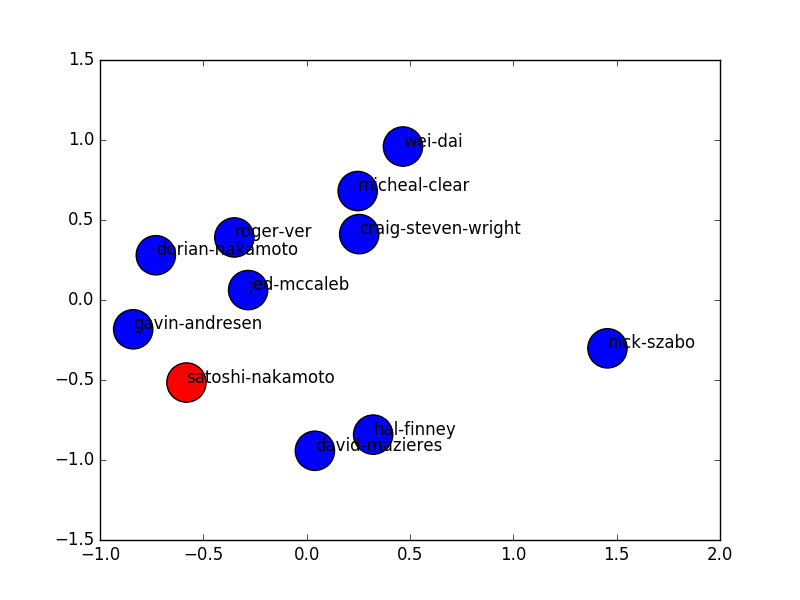
\includegraphics[width=1.4\textwidth]{figure_4}}
\caption{Experiment 4: 4 dimensional author embedding, 95 dimension word embedding, trained for 48 hours. Minimum sentence length is 5}
\end{figure}
\begin{figure}
\noindent\makebox[\textwidth]{%
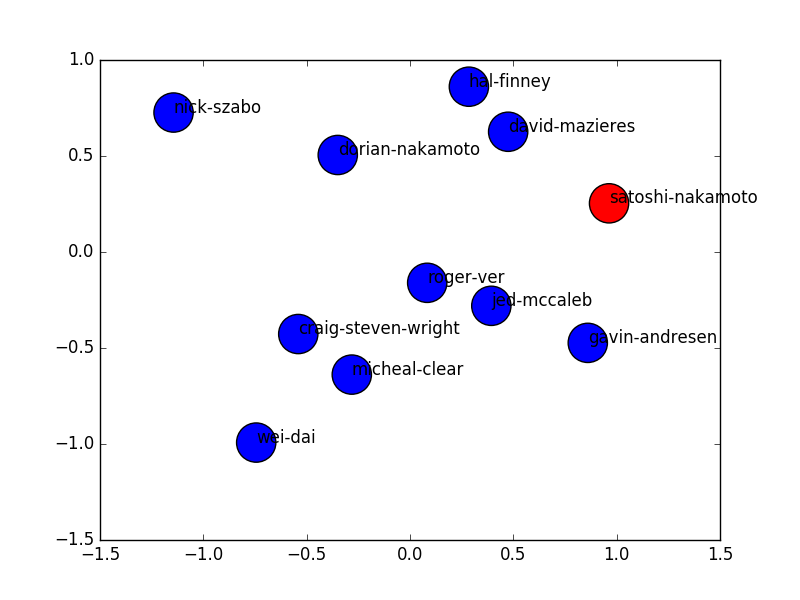
\includegraphics[width=1.4\textwidth]{figure_5}}
\caption{Experiment 5: 5 dimensional author embedding, 65 dimension word embedding, trained for 48 hours. Minimum sentence length is 5}
\end{figure}
\begin{figure}
\noindent\makebox[\textwidth]{%
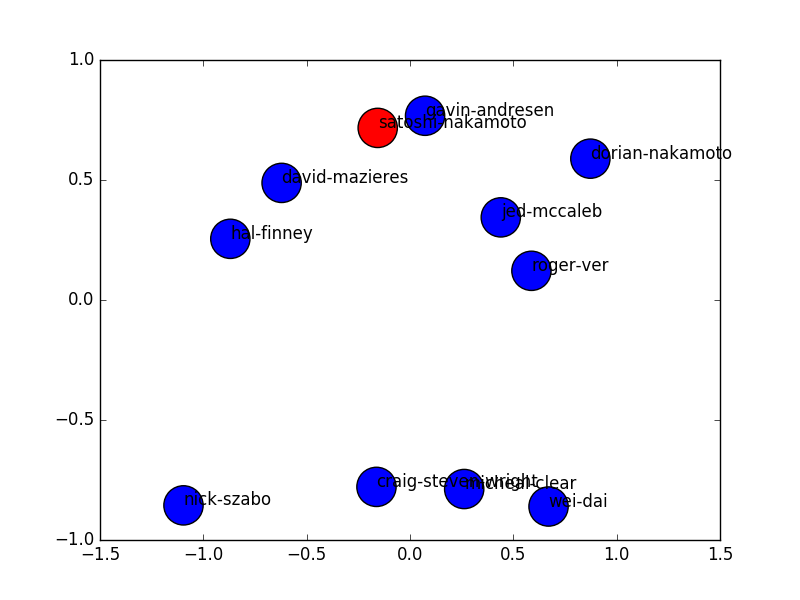
\includegraphics[width=1.4\textwidth]{figure_6}}
\caption{Experiment 6: 5 dimensional author embedding, 65 dimension word embedding, trained for 48 hours. Minimum sentence length is 5}
\end{figure}
\begin{figure}
\noindent\makebox[\textwidth]{%
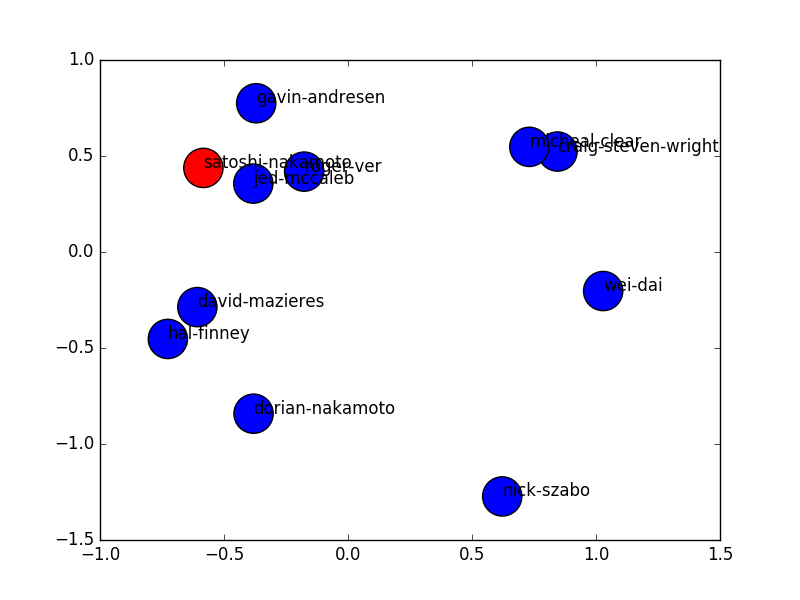
\includegraphics[width=1.4\textwidth]{figure_7}}
\caption{Experiment 7: 4 dimensional author embedding, 85 dimension word embedding, trained for 48 hours. Minimum sentence length is 5}
\end{figure}
\begin{figure}
\noindent\makebox[\textwidth]{%
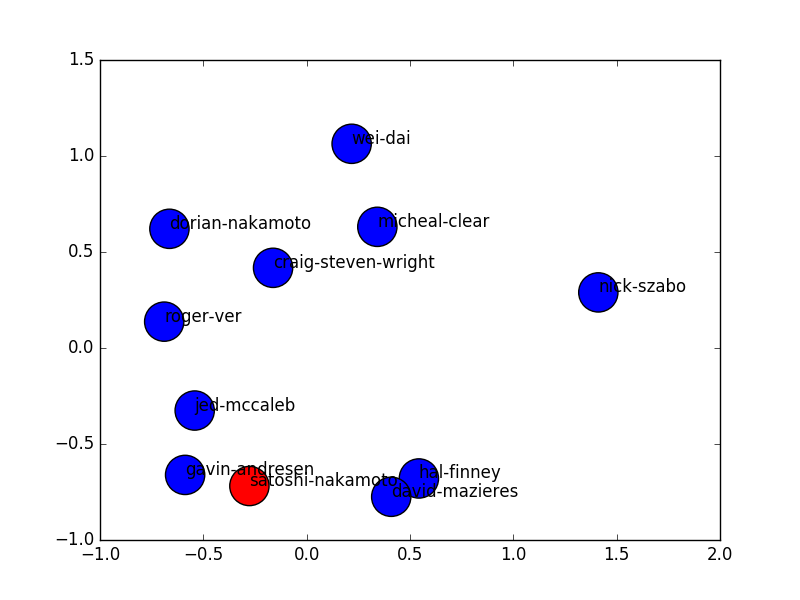
\includegraphics[width=1.4\textwidth]{figure_8}}
\caption{Experiment 8: 4 dimensional author embedding, 110 dimension word embedding, trained for 48 hours. Minimum sentence length is 5}
\end{figure}
\begin{figure}
\noindent\makebox[\textwidth]{%
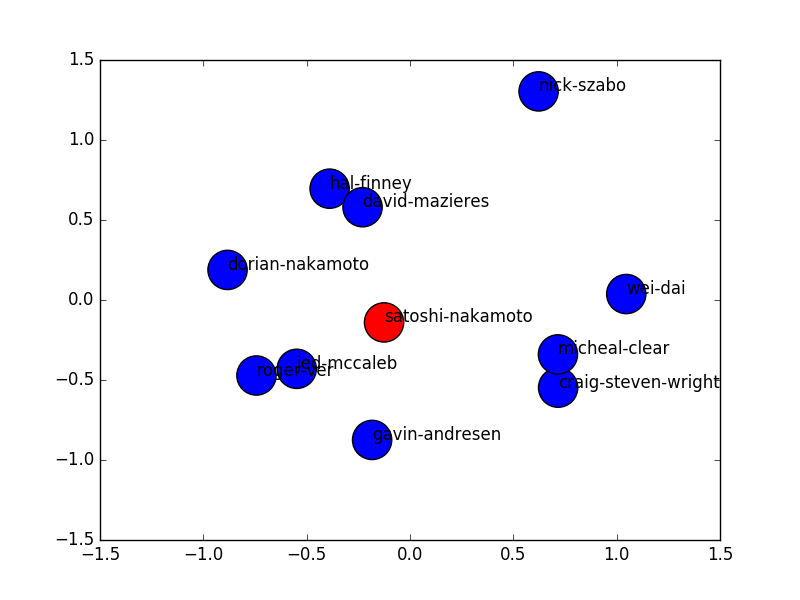
\includegraphics[width=1.4\textwidth]{figure_9}}
\caption{Experiment 9: 5 dimensional author embedding, 110 dimension word embedding, trained for 48 hours. Minimum sentence length is 5}
\end{figure}
\begin{figure}
\noindent\makebox[\textwidth]{%
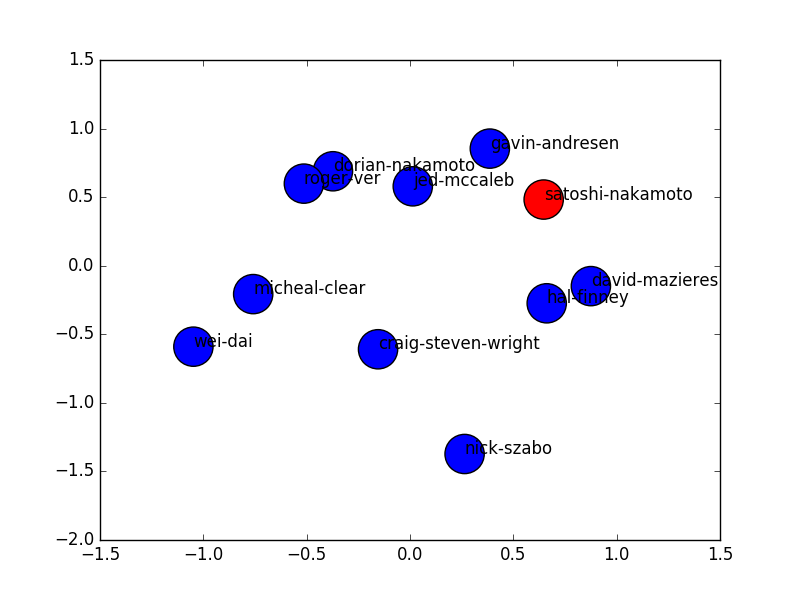
\includegraphics[width=1.4\textwidth]{figure_10}}
\caption{Experiment 10: 6 dimensional author embedding, 40 dimension word embedding, trained for 48 hours. Minimum sentence length is 5}
\end{figure}

\begin{figure}
\noindent\makebox[\textwidth]{%
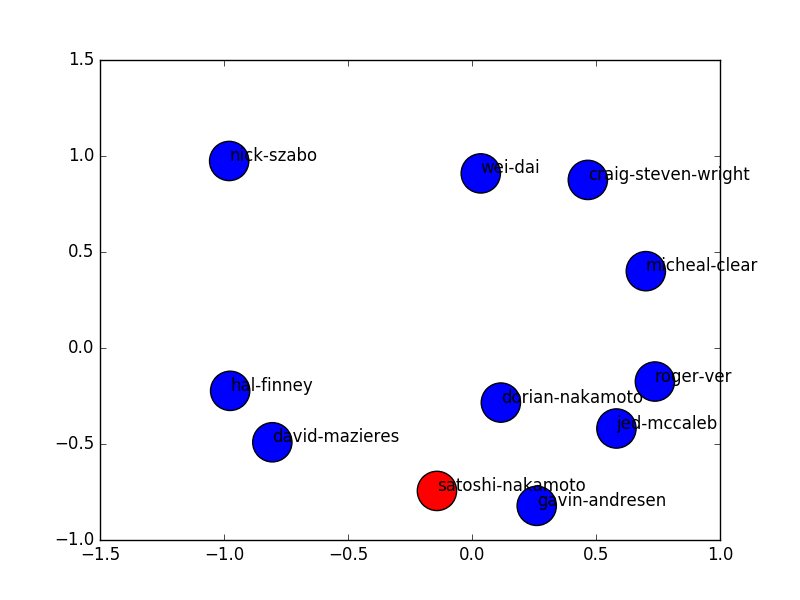
\includegraphics[width=1.4\textwidth]{figure_81}}
\caption{Experiment 11: 6 dimensional author embedding, 90 dimension word embedding, trained for 48 hours. Minimum sentence length is 8}
\end{figure}
\begin{figure}
\noindent\makebox[\textwidth]{%
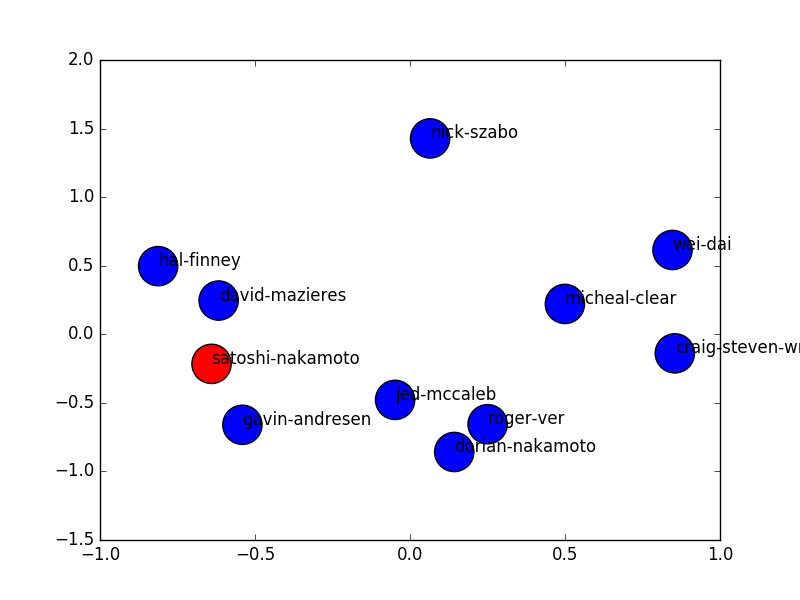
\includegraphics[width=1.4\textwidth]{figure_82}}
\caption{Experiment 12: 6 dimensional author embedding, 90 dimension word embedding, trained for 48 hours. Minimum sentence length is 8}
\end{figure}

\begin{figure}
\noindent\makebox[\textwidth]{%
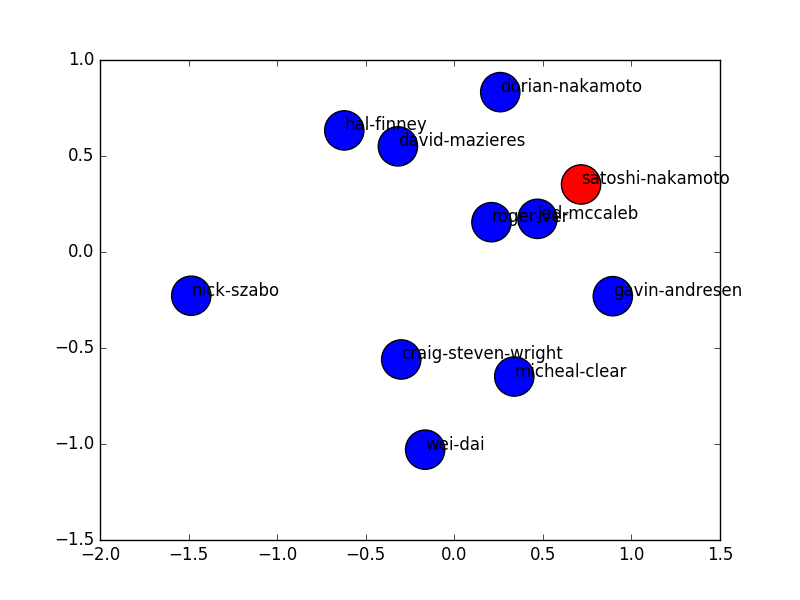
\includegraphics[width=1.4\textwidth]{figure_83}}
\caption{Experiment 13: 4 dimensional author embedding, 90 dimension word embedding, trained for 48 hours. Minimum sentence length is 8}
\end{figure}
\begin{figure}
\noindent\makebox[\textwidth]{%
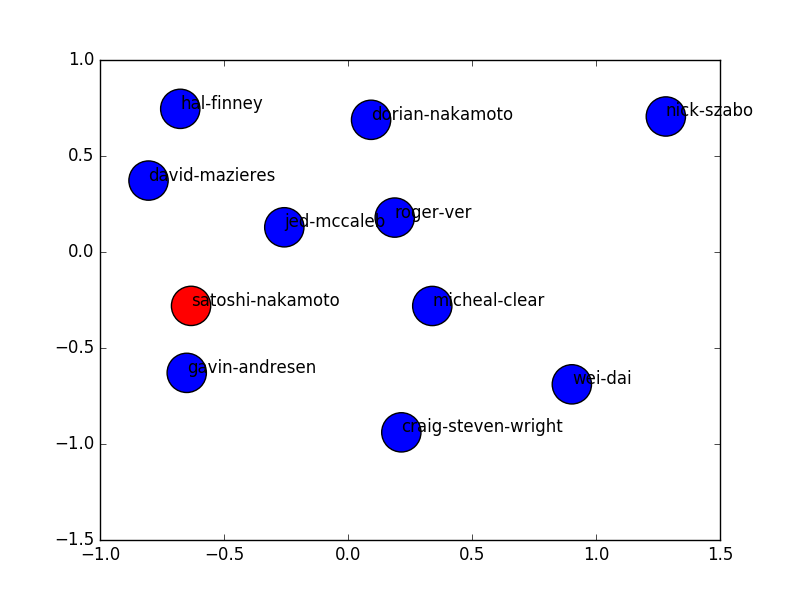
\includegraphics[width=1.4\textwidth]{figure_84}}
\caption{Experiment 14: 7 dimensional author embedding, 80 dimension word embedding, trained for 48 hours. Minimum sentence length is 8}
\end{figure}

\begin{figure}
\noindent\makebox[\textwidth]{%
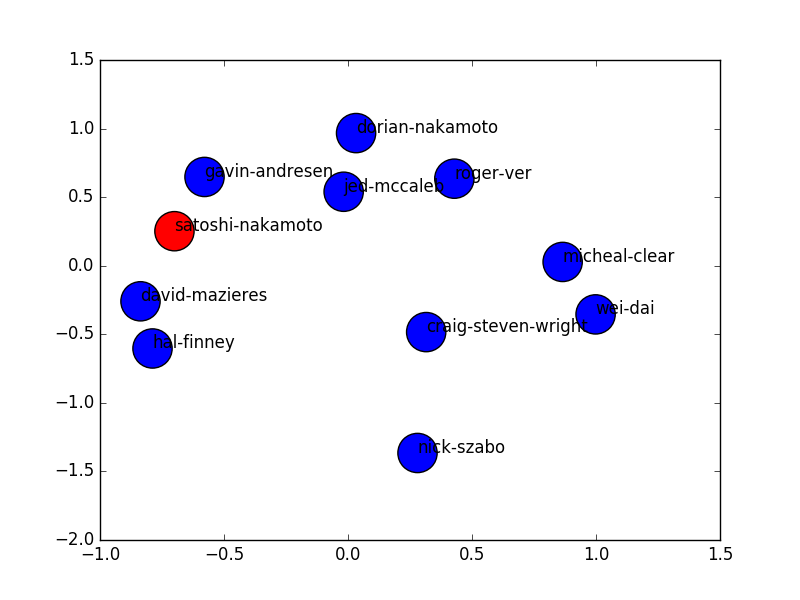
\includegraphics[width=1.4\textwidth]{figure_85}}
\caption{Experiment 15: 6 dimensional author embedding, 105 dimension word embedding, trained for 48 hours. Minimum sentence length is 8}
\end{figure}
\begin{figure}
\noindent\makebox[\textwidth]{%
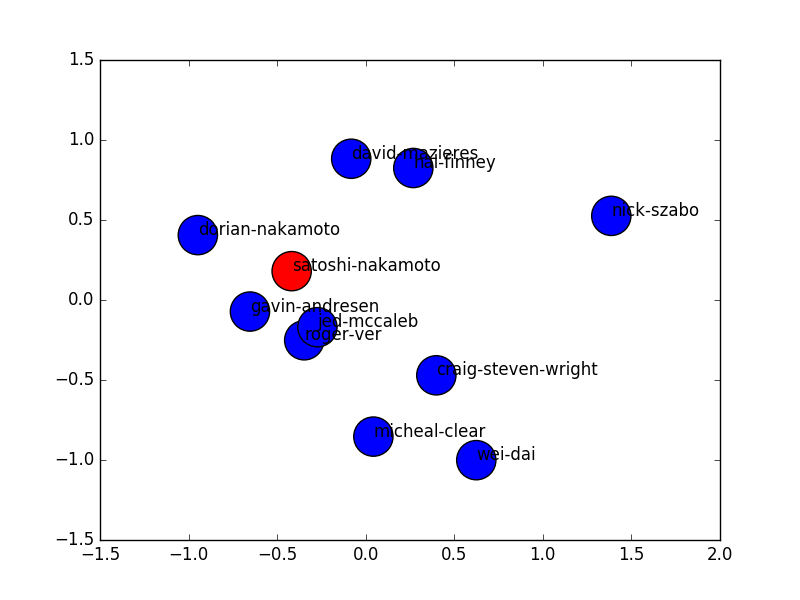
\includegraphics[width=1.4\textwidth]{figure_86}}
\caption{Experiment 16: 4 dimensional author embedding, 100 dimension word embedding, trained for 48 hours. Minimum sentence length is 8}
\end{figure}






\end{document}